%!TEX root = ../../Main.tex
\graphicspath{{Chapters/Identifikation_af_open_loop_system/}}
%-------------------------------------------------------------------------------

\section{Identifikation af open-loop system}

Efter vi har besluttet os på hvilket system vi ønskede at designe, og hvilke dele det skal bestå af, er det næste skridt at indsamle data fra vores motor via den indlagte encoder. Det gør vi ved at sende et step input ind på motoren. Vi aflæser to outputs, både det direkte output fra encoderen, som er rotationen i grader, samt den afledte som er hastigheden i grader. Opstillingen af denne måling i Simulink kan ses på \autoref{fig:Simulink_opstilling_af_maaling}. Disse målinger gentog vi mange gange, for at få de bedst mulige målinger. Grunden til at vi ønsker de bedste mulige målinger er, så vi kan lave den bedst mulige repræsentation af vores system, så det system vi beregner på, er så tæt på det faktiske system som overhovedet muligt.
  
\begin{figure}[H]
	\centering
	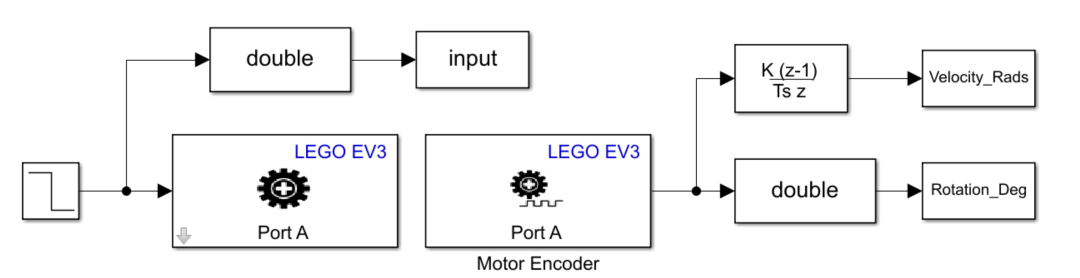
\includegraphics[width = 400pt]{Img/Simulink_opstilling_af_maaling.png}
	\caption{Simulink opstilling af måling}
	\label{fig:Simulink_opstilling_af_maaling}
\end{figure}

Grafen på \autoref{fig:Motor_deg_graf} repræsenterer motorens rotation i grader. Grafen på \autoref{fig:Motor_velocity_graf} repræsenterer den afledte af rotation i grader, altså hastigheden i grader. Som man kan se på \autoref{fig:Motor_velocity_graf} opfører den afledte sig som et første ordens system, dog med et lille udfald i accelerationen, men da den er så lille vælger vi at se bort fra denne. Da vores afledte opfører sig som et første ordens system må det betyde at vores system er et 2. ordens system. 

\begin{figure}[H]
	\centering
	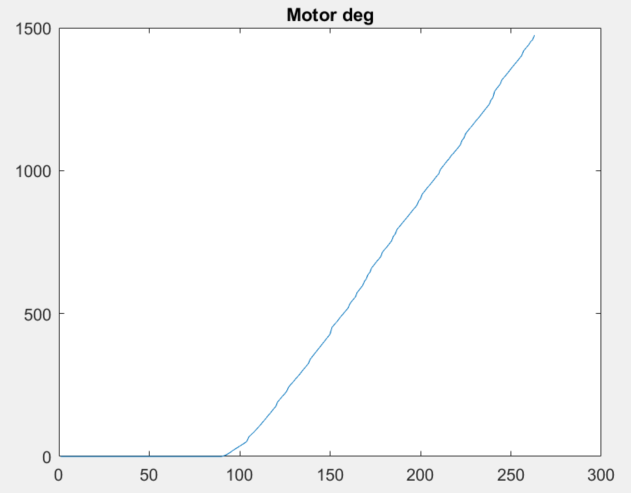
\includegraphics[width = 300pt]{Img/Motor_deg_graf.png}
	\caption{Måling af motor vinkel i grader}
	\label{fig:Motor_deg_graf}
\end{figure}

\begin{figure}[H]
	\centering
	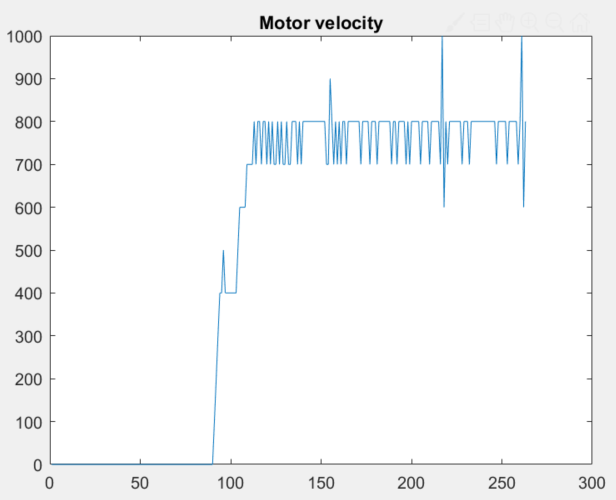
\includegraphics[width = 300pt]{Img/Motor_velocity_graf.png}
	\caption{Måling af motor vinkel i hastighed}
	\label{fig:Motor_velocity_graf}
\end{figure}





\newpage